
% \iffalse
% \begin{table*}[ht] 
%     \centering 
%     \begin{tabular}{lcp{18mm}p{14mm}p{15mm}p{10mm}p{16mm}cc} 
%         \textbf{Method} & \textbf{Orthogonal} & \textbf{Equivalent Kernel Size} & \textbf{Code available} & \textbf{Change Channels} & \textbf{Stride} & \textbf{Conv Transpose} & \textbf{Groups} & \textbf{Dilation}\\
%         \hline 
%         BCOP \cite{singla_skew_2021} & \cmark & $k$ & \cmark & \cmark & $\capprox$ & \xmark & \xmark & \xmark \\
%         SC-FAC \cite{su_scaling-up_2021} & \cmark & $k$ separable & \xmark & \cmark &  \cmark & $\capprox$ & \cmark & \cmark \\
%         ECO \cite{yu_constructing_2021} & \cmark & $I_w \times I_h$ & \xmark & $\capprox$ & $\capprox$ & \xmark & \xmark & $\capprox$ \\
%         Cayley \cite{trockman_orthogonalizing_2021} & \cmark & $I_w \times I_h$ & \cmark & $\capprox$ & $\capprox$ & $\capprox$ & \xmark & \xmark \\
%         LOT \cite{xu_lot_2023} & \cmark & $I_w \times I_h$ & \cmark & \cmark & $\capprox$ & \xmark & \xmark & \xmark \\
%         ProjUNN-T \cite{kiani_projunn_2022} & \cmark & $I_w \times I_h$ & \cmark & \xmark & \xmark & \xmark & \xmark & \xmark\\
%         SLL \cite{araujo_unified_2023} & \xmark & composed & \cmark & \xmark & \xmark & \xmark & \xmark  & \xmark\\
%         Sandwich \cite{wang_direct_2023} & \xmark & composed & \cmark & $\capprox$ & $\capprox$ & \xmark & \xmark  & \xmark\\
%         AOL \cite{prach_almost-orthogonal_2022} & \xmark & $k$ & \cmark & \cmark & \cmark & \xmark & \xmark & \xmark \\
%         SOC \cite{singla_skew_2021} & \cmark & $k + (n\frac{k}{2})$ & \cmark & $\capprox$ & $\capprox$ & \xmark & \xmark & \xmark \\
%         \hline
%         \textbf{AOC (Ours)} & \cmark & $k$ & \cmark & \cmark & \cmark & \cmark & \cmark & \cmark \\
%     \end{tabular}
%     \caption{\thib{TODO: gérer le format de citations}\textbf{Comparison of orthogonal convolution methods.} A check mark (\cmark) indicates full support for the feature, a cross mark (\xmark) indicates lack of support (in the implementation), and an approximate symbol ($\approx$) indicates partial support (emulation). Here, $k$ denotes the kernel size, and $I_w \times I_h$ represents the input dimensions. AOC is the first method to support strides, dilations, group convolution and transposed convolution. \vspace{-4mm}}
%     \label{tab:big_picture}
% \end{table*}

% \fi

\begin{table*}[ht] 
    \centering 
    \begin{tabular}{llcp{16mm}cccccc} 
        \textbf{Method} & &\rotatebox[origin=c]{80}{\textbf{Orthogonal}} & \rotatebox[origin=c]{80}{\parbox[c]{16mm}{\centering \textbf{Equivalent Kernel Size}}} & \rotatebox[origin=c]{80}{\parbox[c]{16mm}{\centering \textbf{Code available}}} & \rotatebox[origin=c]{80}{\parbox[c]{16mm}{\centering \textbf{Change Channels}}} & \rotatebox[origin=c]{80}{\textbf{Stride}} & \rotatebox[origin=c]{80}{\parbox[c]{16mm}{\centering \textbf{Conv Transpose}}} & \rotatebox[origin=c]{80}{\textbf{Groups}} & \rotatebox[origin=c]{80}{\textbf{Dilation}}\\
        \hline 
        BCOP &\cite{li_preventing_2019} & \cmark & $k$ & \cmark & \cmark & $\capprox$ & \xmark & \xmark & \xmark \\
        SC-FAC &\cite{su_scaling-up_2021} & \cmark & $k$ separable & \xmark & \cmark &  \cmark & $\capprox$ & \cmark & \cmark \\
        ECO &\cite{yu_constructing_2021} & \cmark & $I_w \times I_h$ & \xmark & $\capprox$ & $\capprox$ & \xmark & \xmark & $\capprox$ \\
        Cayley &\cite{trockman_orthogonalizing_2021} & \cmark & $I_w \times I_h$ & \cmark & $\capprox$ & $\capprox$ & $\capprox$ & \xmark & \xmark \\
        LOT &\cite{xu_lot_2023} & \cmark & $I_w \times I_h$ & \cmark & \cmark & $\capprox$ & \xmark & \xmark & \xmark \\
        ProjUNN-T &\cite{kiani_projunn_2022} & \cmark & $I_w \times I_h$ & \cmark & \xmark & \xmark & \xmark & \xmark & \xmark\\
        SLL &\cite{araujo_unified_2023} & \xmark & composed & \cmark & \xmark & \xmark & \xmark & \xmark  & \xmark\\
        Sandwich &\cite{wang_direct_2023} & \xmark & composed & \cmark & $\capprox$ & $\capprox$ & \xmark & \xmark  & \xmark\\
        AOL &\cite{prach_almost-orthogonal_2022} & \xmark & $k$ & \cmark & \cmark & \cmark & \xmark & \xmark & \xmark \\
        SOC &\cite{singla_skew_2021} & \cmark & $k + (n\frac{k}{2})$ & \cmark & $\capprox$ & $\capprox$ & \xmark & \xmark & \xmark \\
        \hline
        \textbf{AOC}  & \textbf{(Ours)} & \cmark & $k$ & \cmark & \cmark & \cmark & \cmark & \cmark & \cmark \\
    \end{tabular}
    \caption{\textbf{Comparison of orthogonal convolution methods.} A check mark (\cmark) indicates full support for the feature, a cross mark (\xmark) indicates lack of support (in the implementation), and an approximate symbol ($\capprox$) indicates partial support (emulation). Here, $k$ denotes the kernel size, and $I_w \times I_h$ represents the input dimensions. The pip package of AOC provides an implementation supporting strides, dilations, group convolution and transposed convolution. This work also covers the conditions under which other methods could support those features.  %\thib{Emphasize that we looked at implementations, not the methods itself. cf reviewer: Table 1 makes it seem like the proposed method is one of the few methods that allow doing convolutions with groups, dilation and calculate the transpose convolution. I believe that all methods can trivially do grouped convolution, a lot of method can also do dilated convolution and transposed convolution. For fairness it is mentioned that this table is comparing the implementations of the methods, however, I still believe this table is misleading and gives a wrong idea of the contribution of this paper.}
\vspace{-4mm}}
    \label{tab:big_picture}
\end{table*}


% \begin{table*}[ht] 
%     \centering 
%     \begin{tabular}{llcp{16mm}cccccc} 
%         \textbf{Method} & &\rotatebox[origin=c]{80}{\textbf{Orthogonal}} & \rotatebox[origin=c]{80}{\parbox[c]{16mm}{\centering \textbf{Equivalent Kernel Size}}} & \rotatebox[origin=c]{80}{\parbox[c]{16mm}{\centering \textbf{Code available}}} & \rotatebox[origin=c]{80}{\parbox[c]{16mm}{\centering \textbf{Change Channels}}} & \rotatebox[origin=c]{80}{\textbf{Stride}} & \rotatebox[origin=c]{80}{\parbox[c]{16mm}{\centering \textbf{Conv Transpose}}} & \rotatebox[origin=c]{80}{\textbf{Groups}} & \rotatebox[origin=c]{80}{\textbf{Dilation}}\\
%         \hline 
%         BCOP &\cite{li_preventing_2019} & \cmark & $k$ & \cmark & \cmark & $\capprox$ & \xmark & \xmark & \xmark \\
%         % --- ORTHOGONIUM version
%          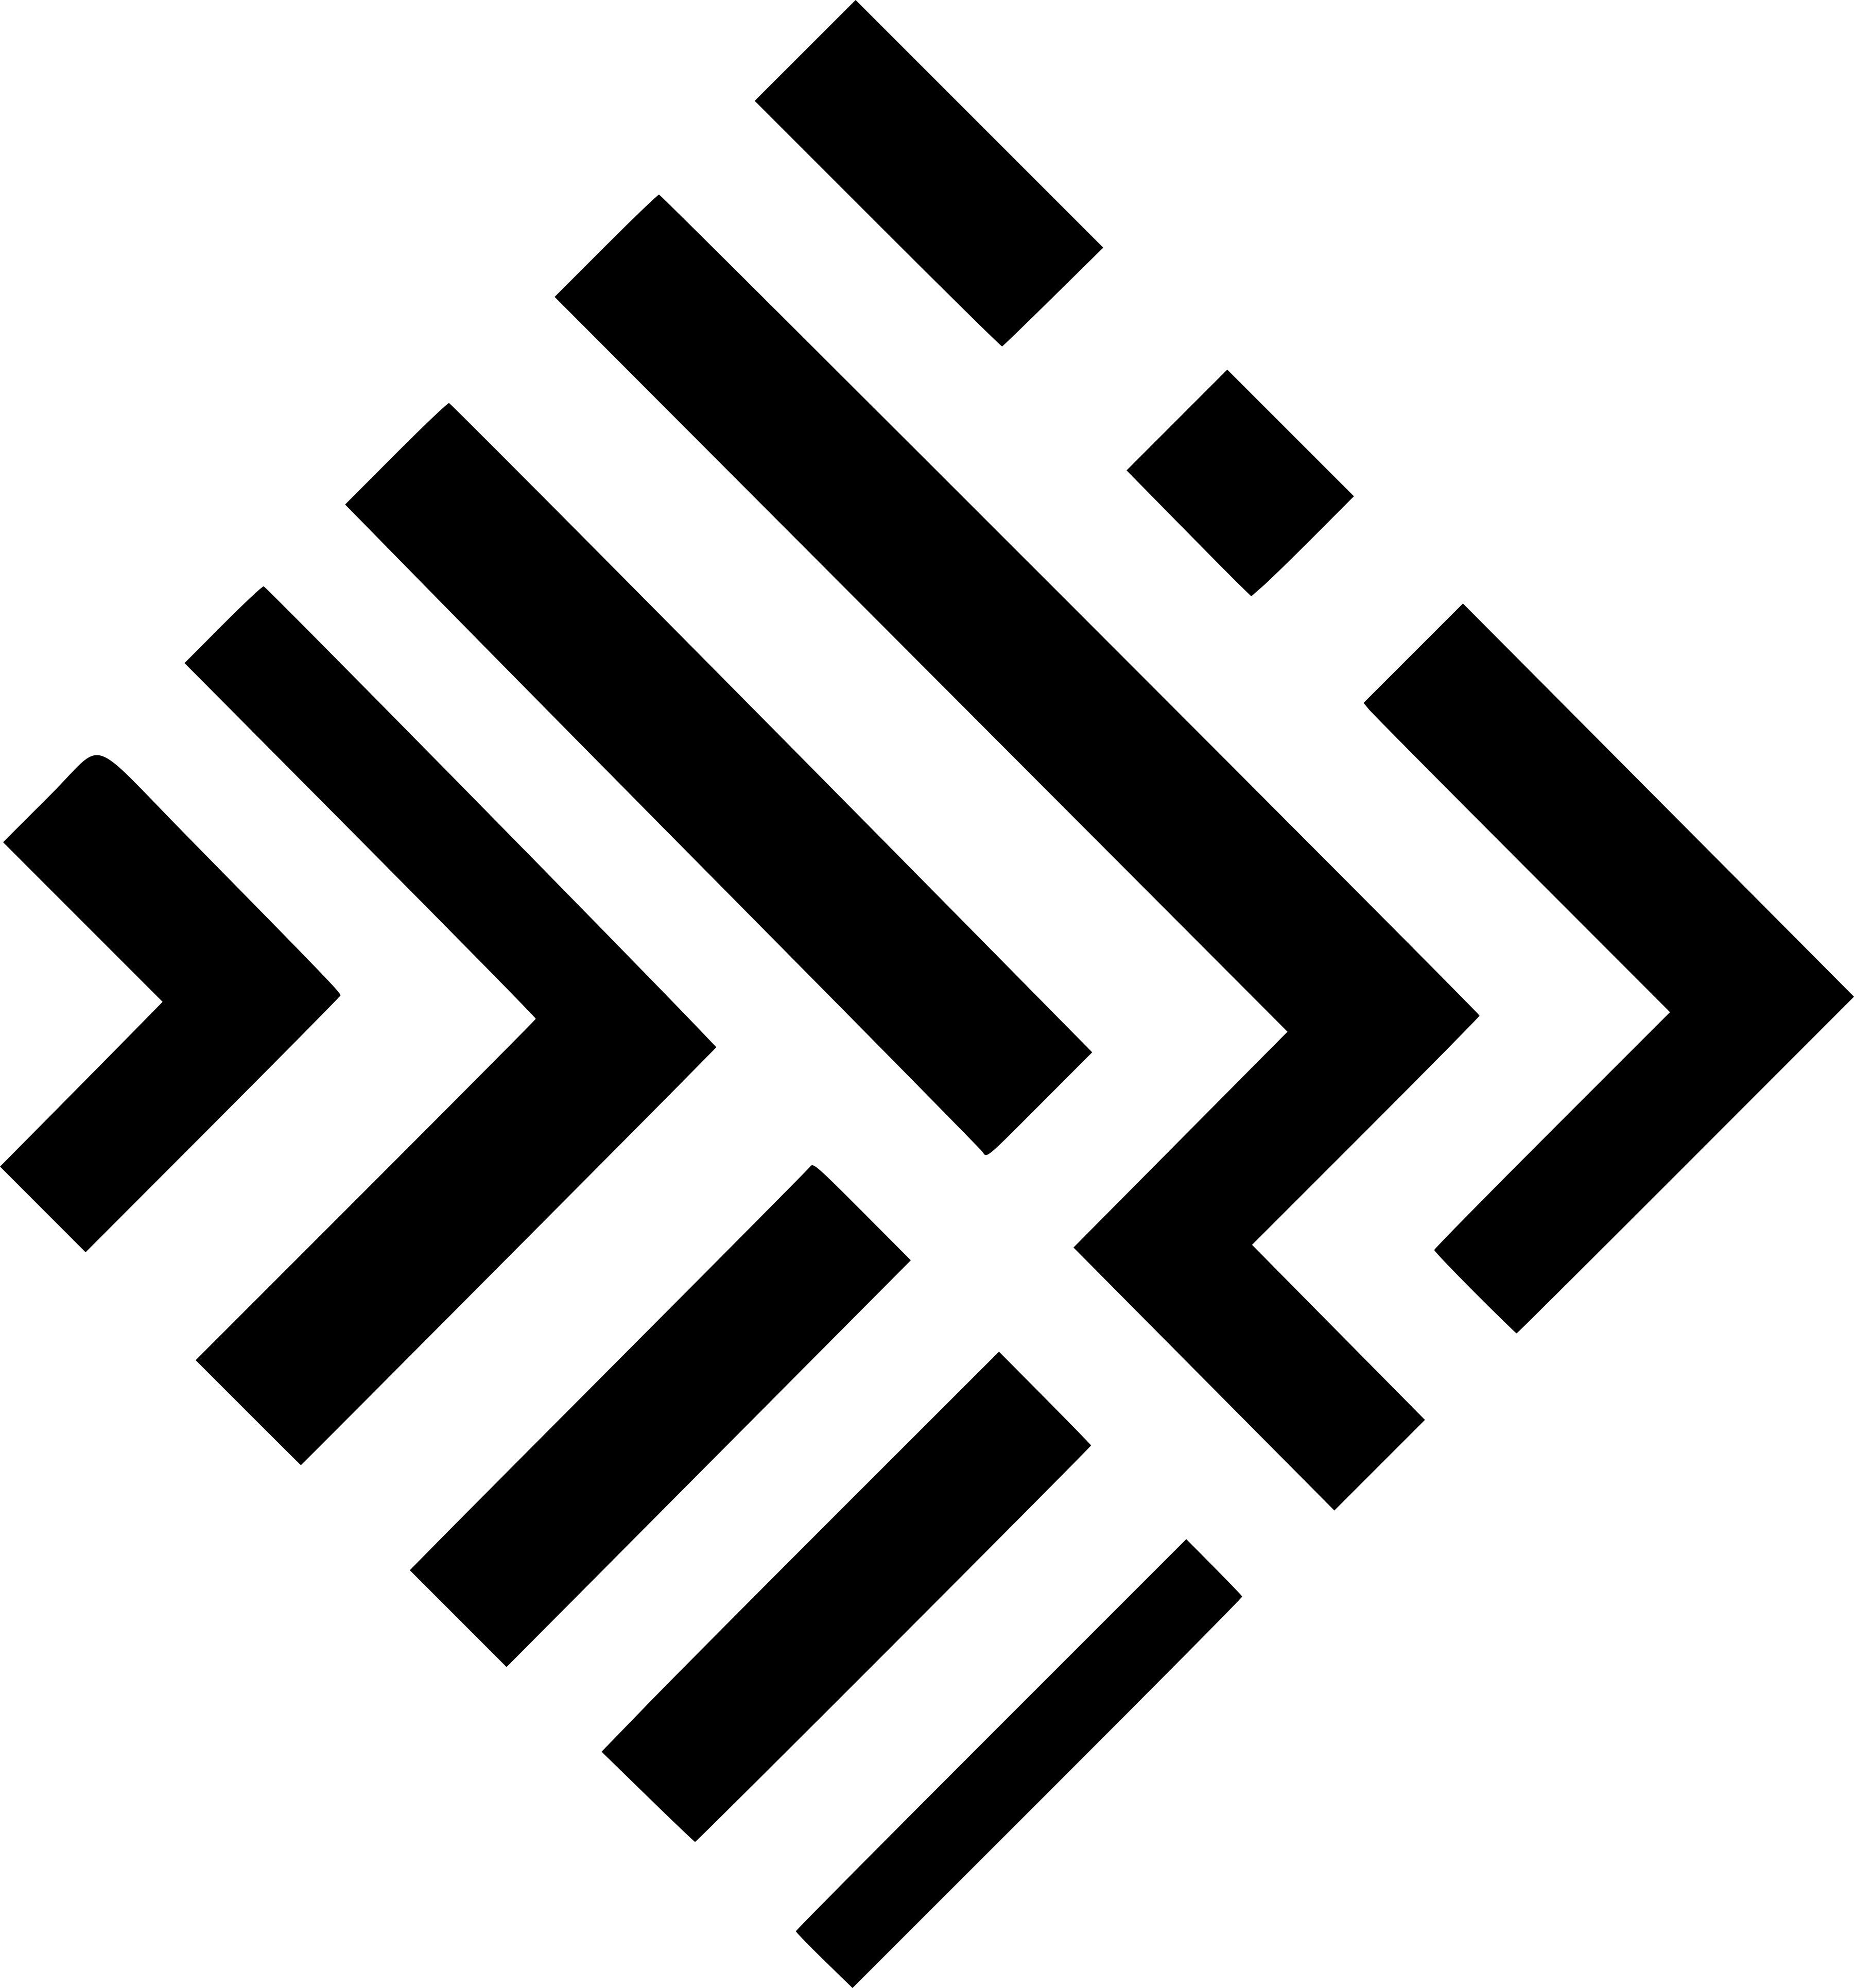
\includegraphics[height=2ex]{figures/ch3_aoc/illustrations/orthogonium_logo_b.png} AOC & & \cmark & $k$ & \cmark & \cmark & \cmark & \cmark & \cmark & \cmark \\

%         SLL &\cite{araujo_unified_2023} & \xmark & composed & \cmark & \xmark & \xmark & \xmark & \xmark  & \xmark\\
%          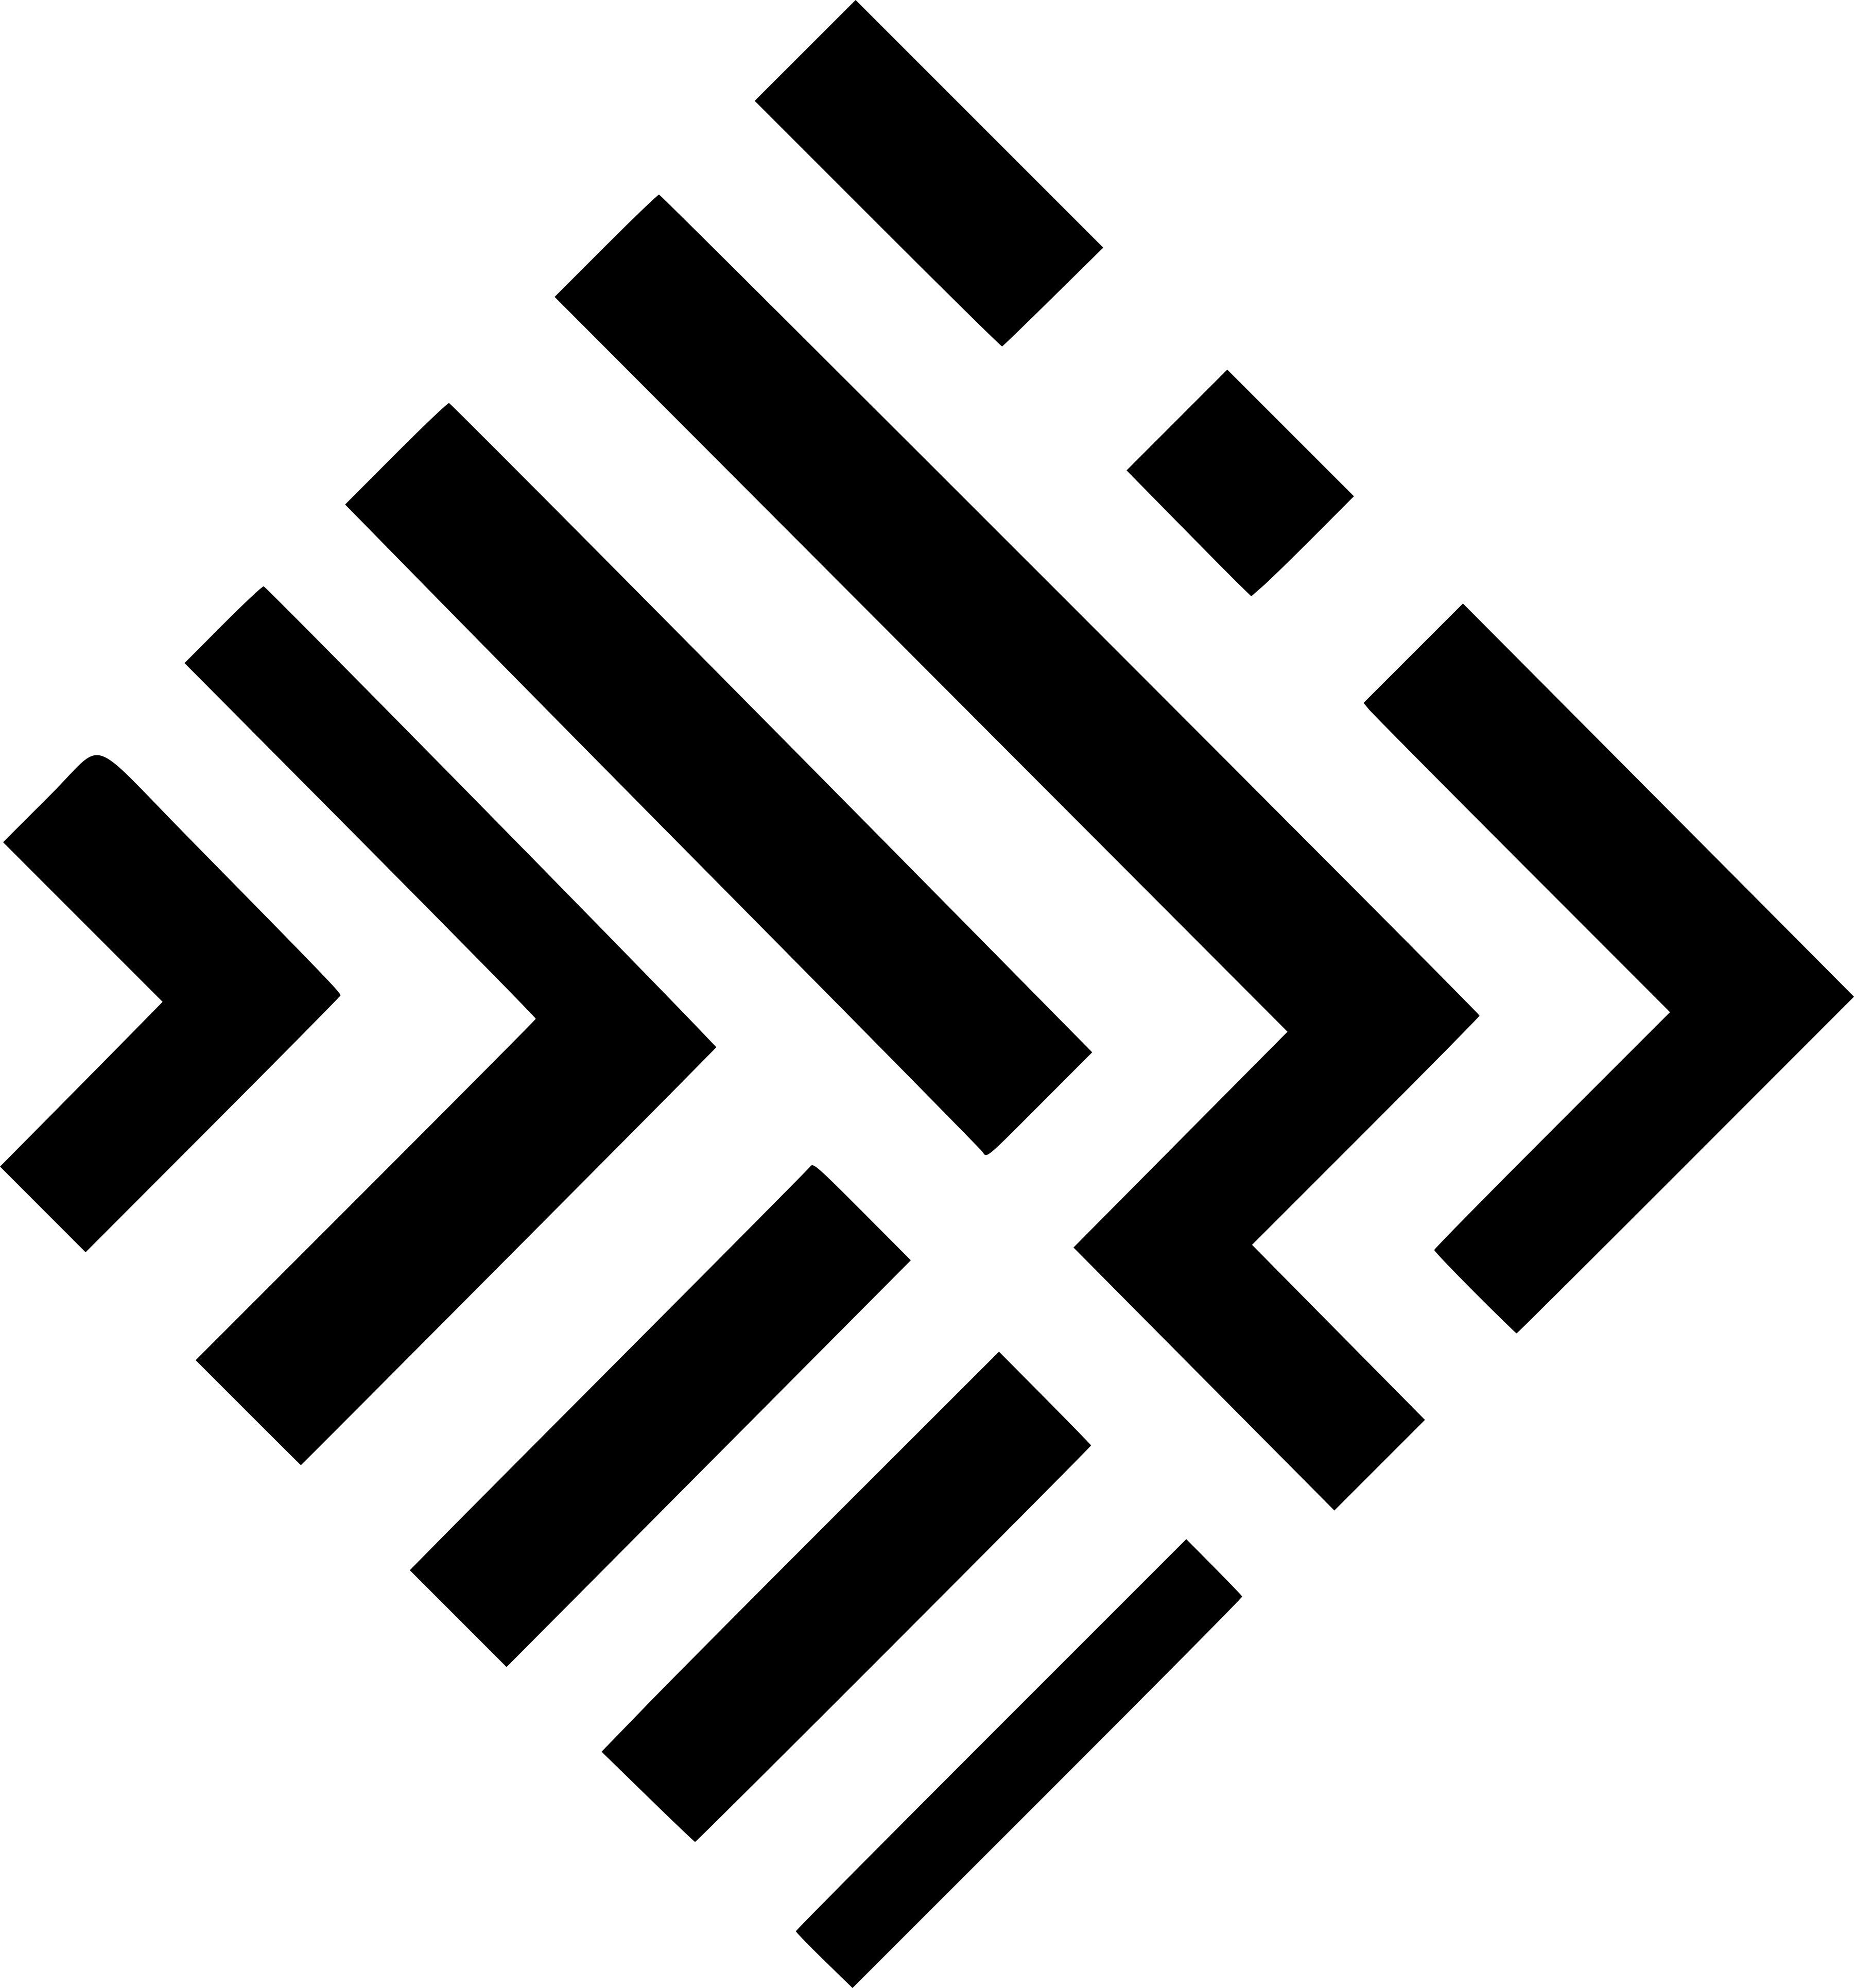
\includegraphics[height=2ex]{figures/ch3_aoc/illustrations/orthogonium_logo_b.png} SLL & & \cmark & composed & \cmark & \cmark & \cmark & \cmark & \cmark  & \cmark\\

%         AOL &\cite{prach_almost-orthogonal_2022} & \xmark & $k$ & \cmark & \cmark & \cmark & \xmark & \xmark & \xmark \\
%         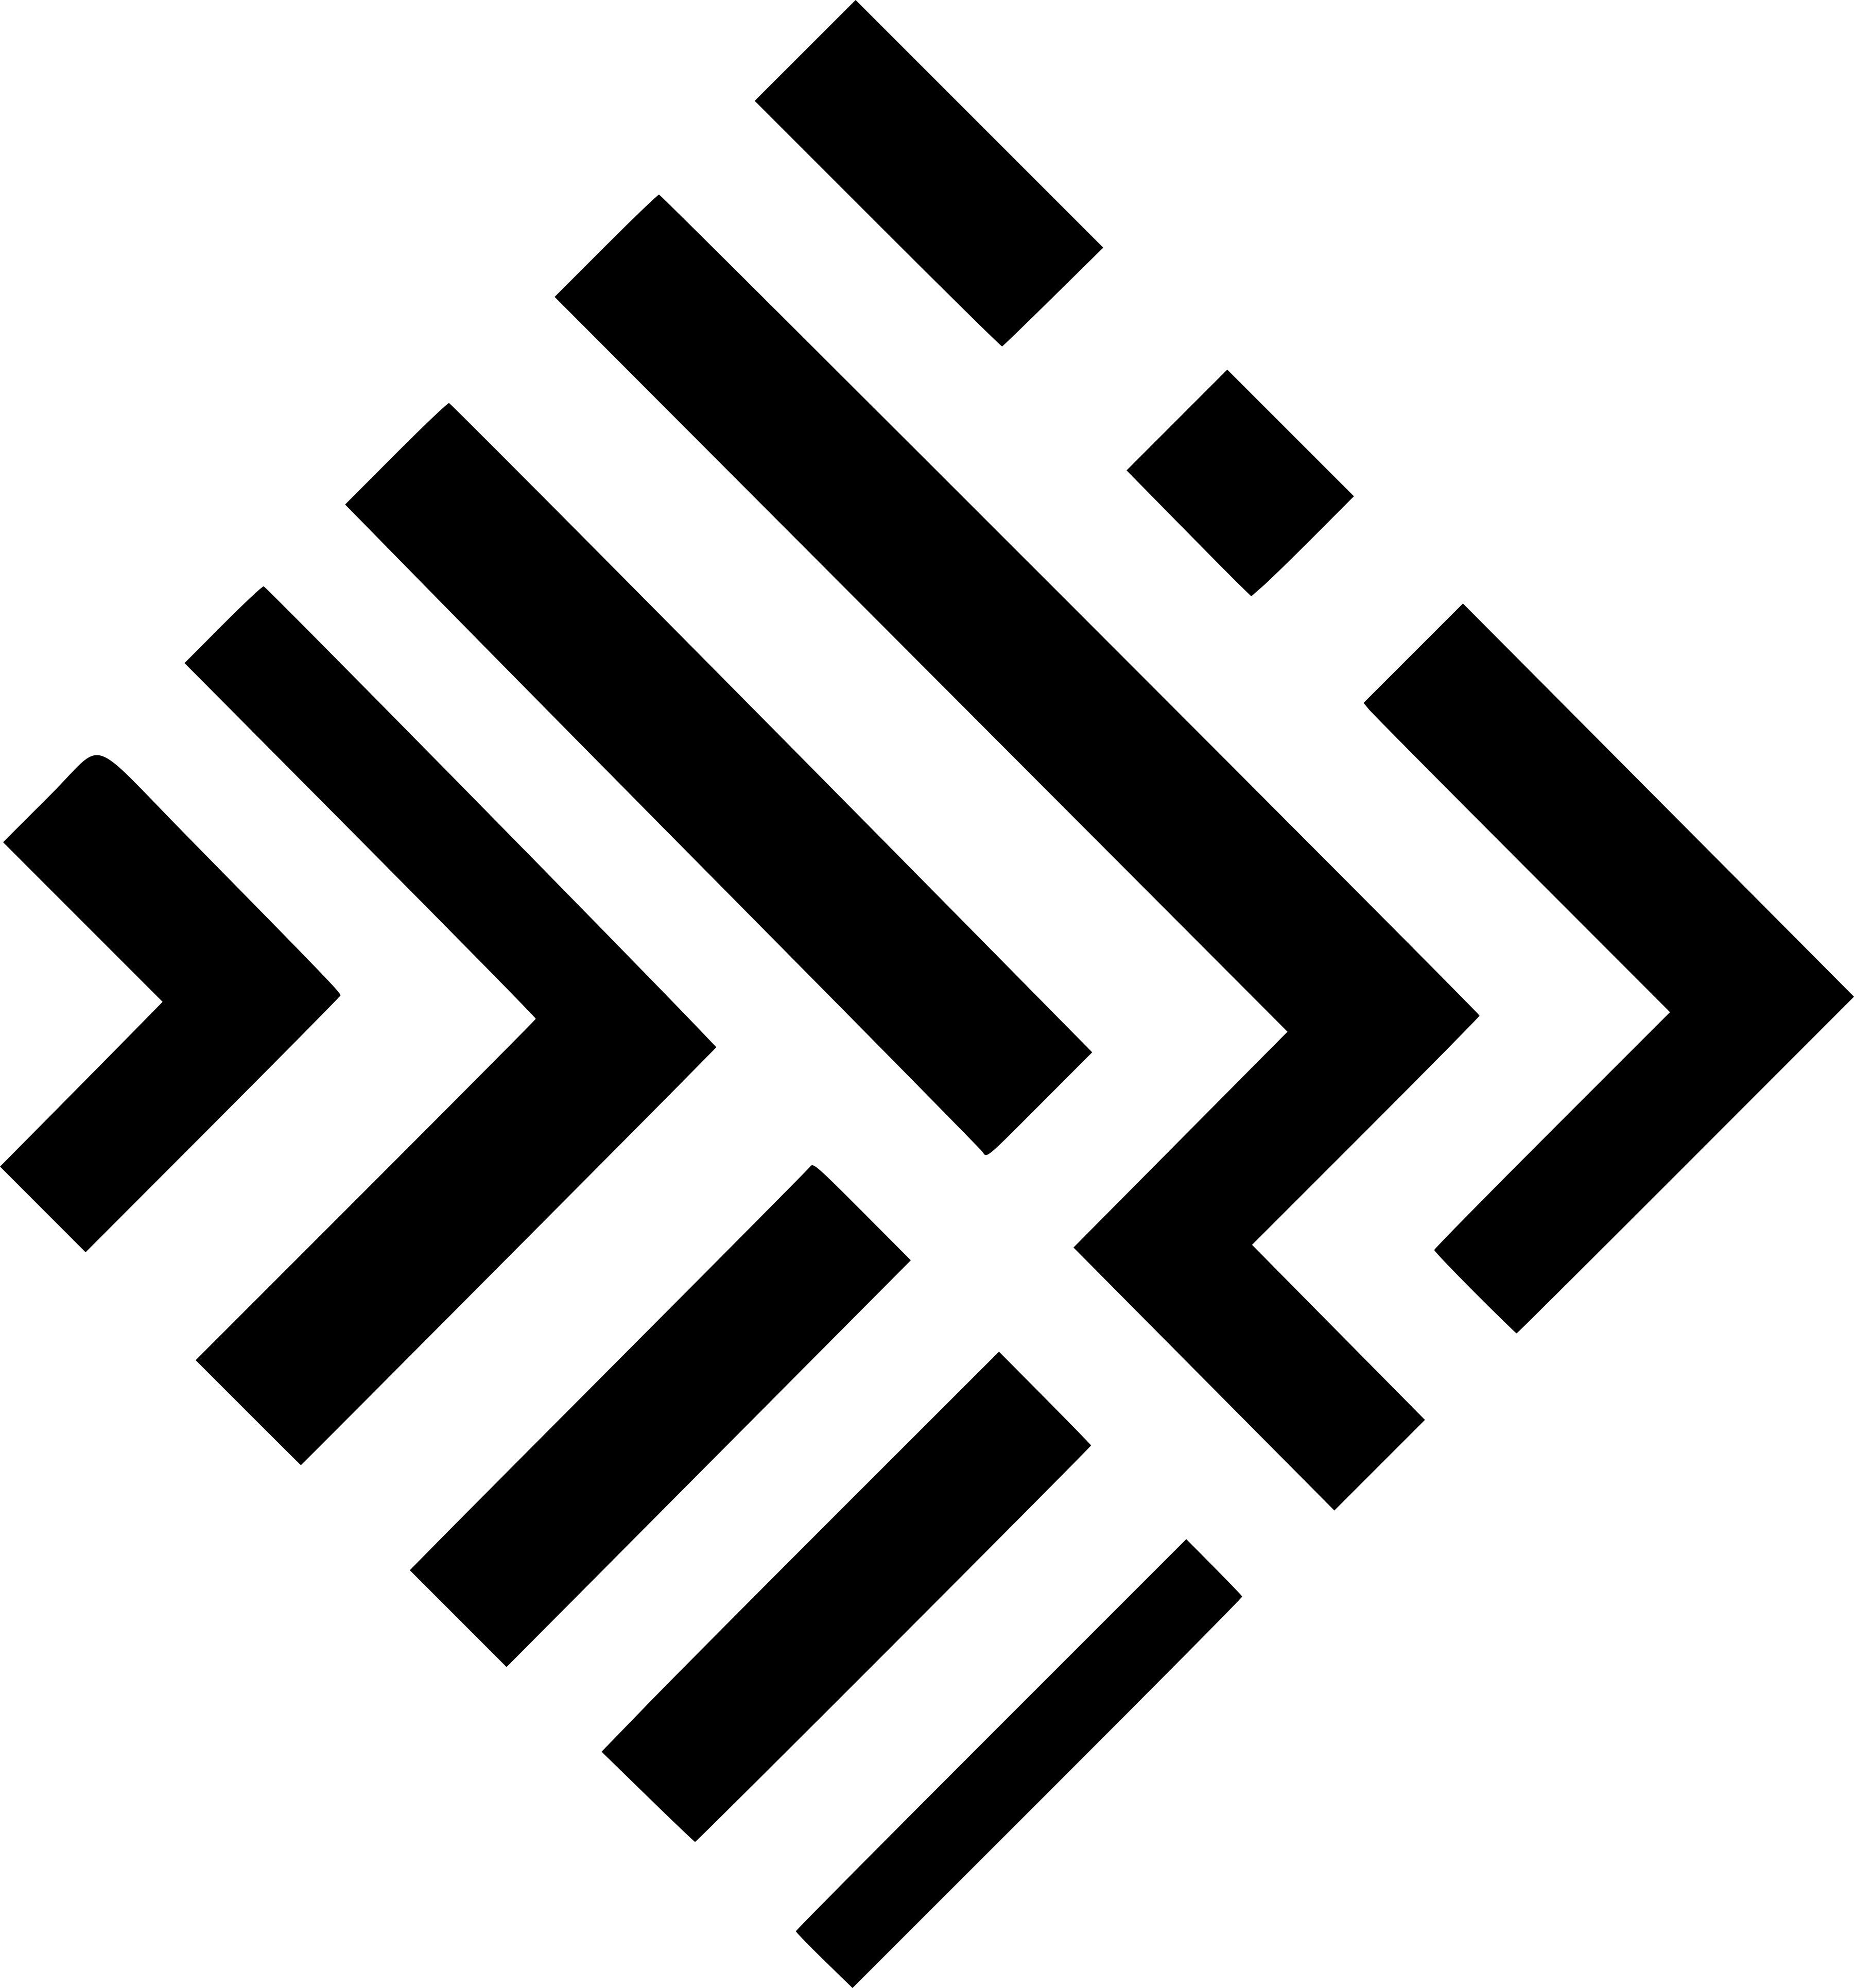
\includegraphics[height=2ex]{figures/ch3_aoc/illustrations/orthogonium_logo_b.png} AOL & & \cmark & $k$ & \cmark & \cmark & \cmark & \cmark & \cmark & \cmark \\

%         SOC &\cite{singla_skew_2021} & \cmark & $k + (n\frac{k}{2})$ & \cmark & $\capprox$ & $\capprox$ & \xmark & \xmark & \xmark \\
%          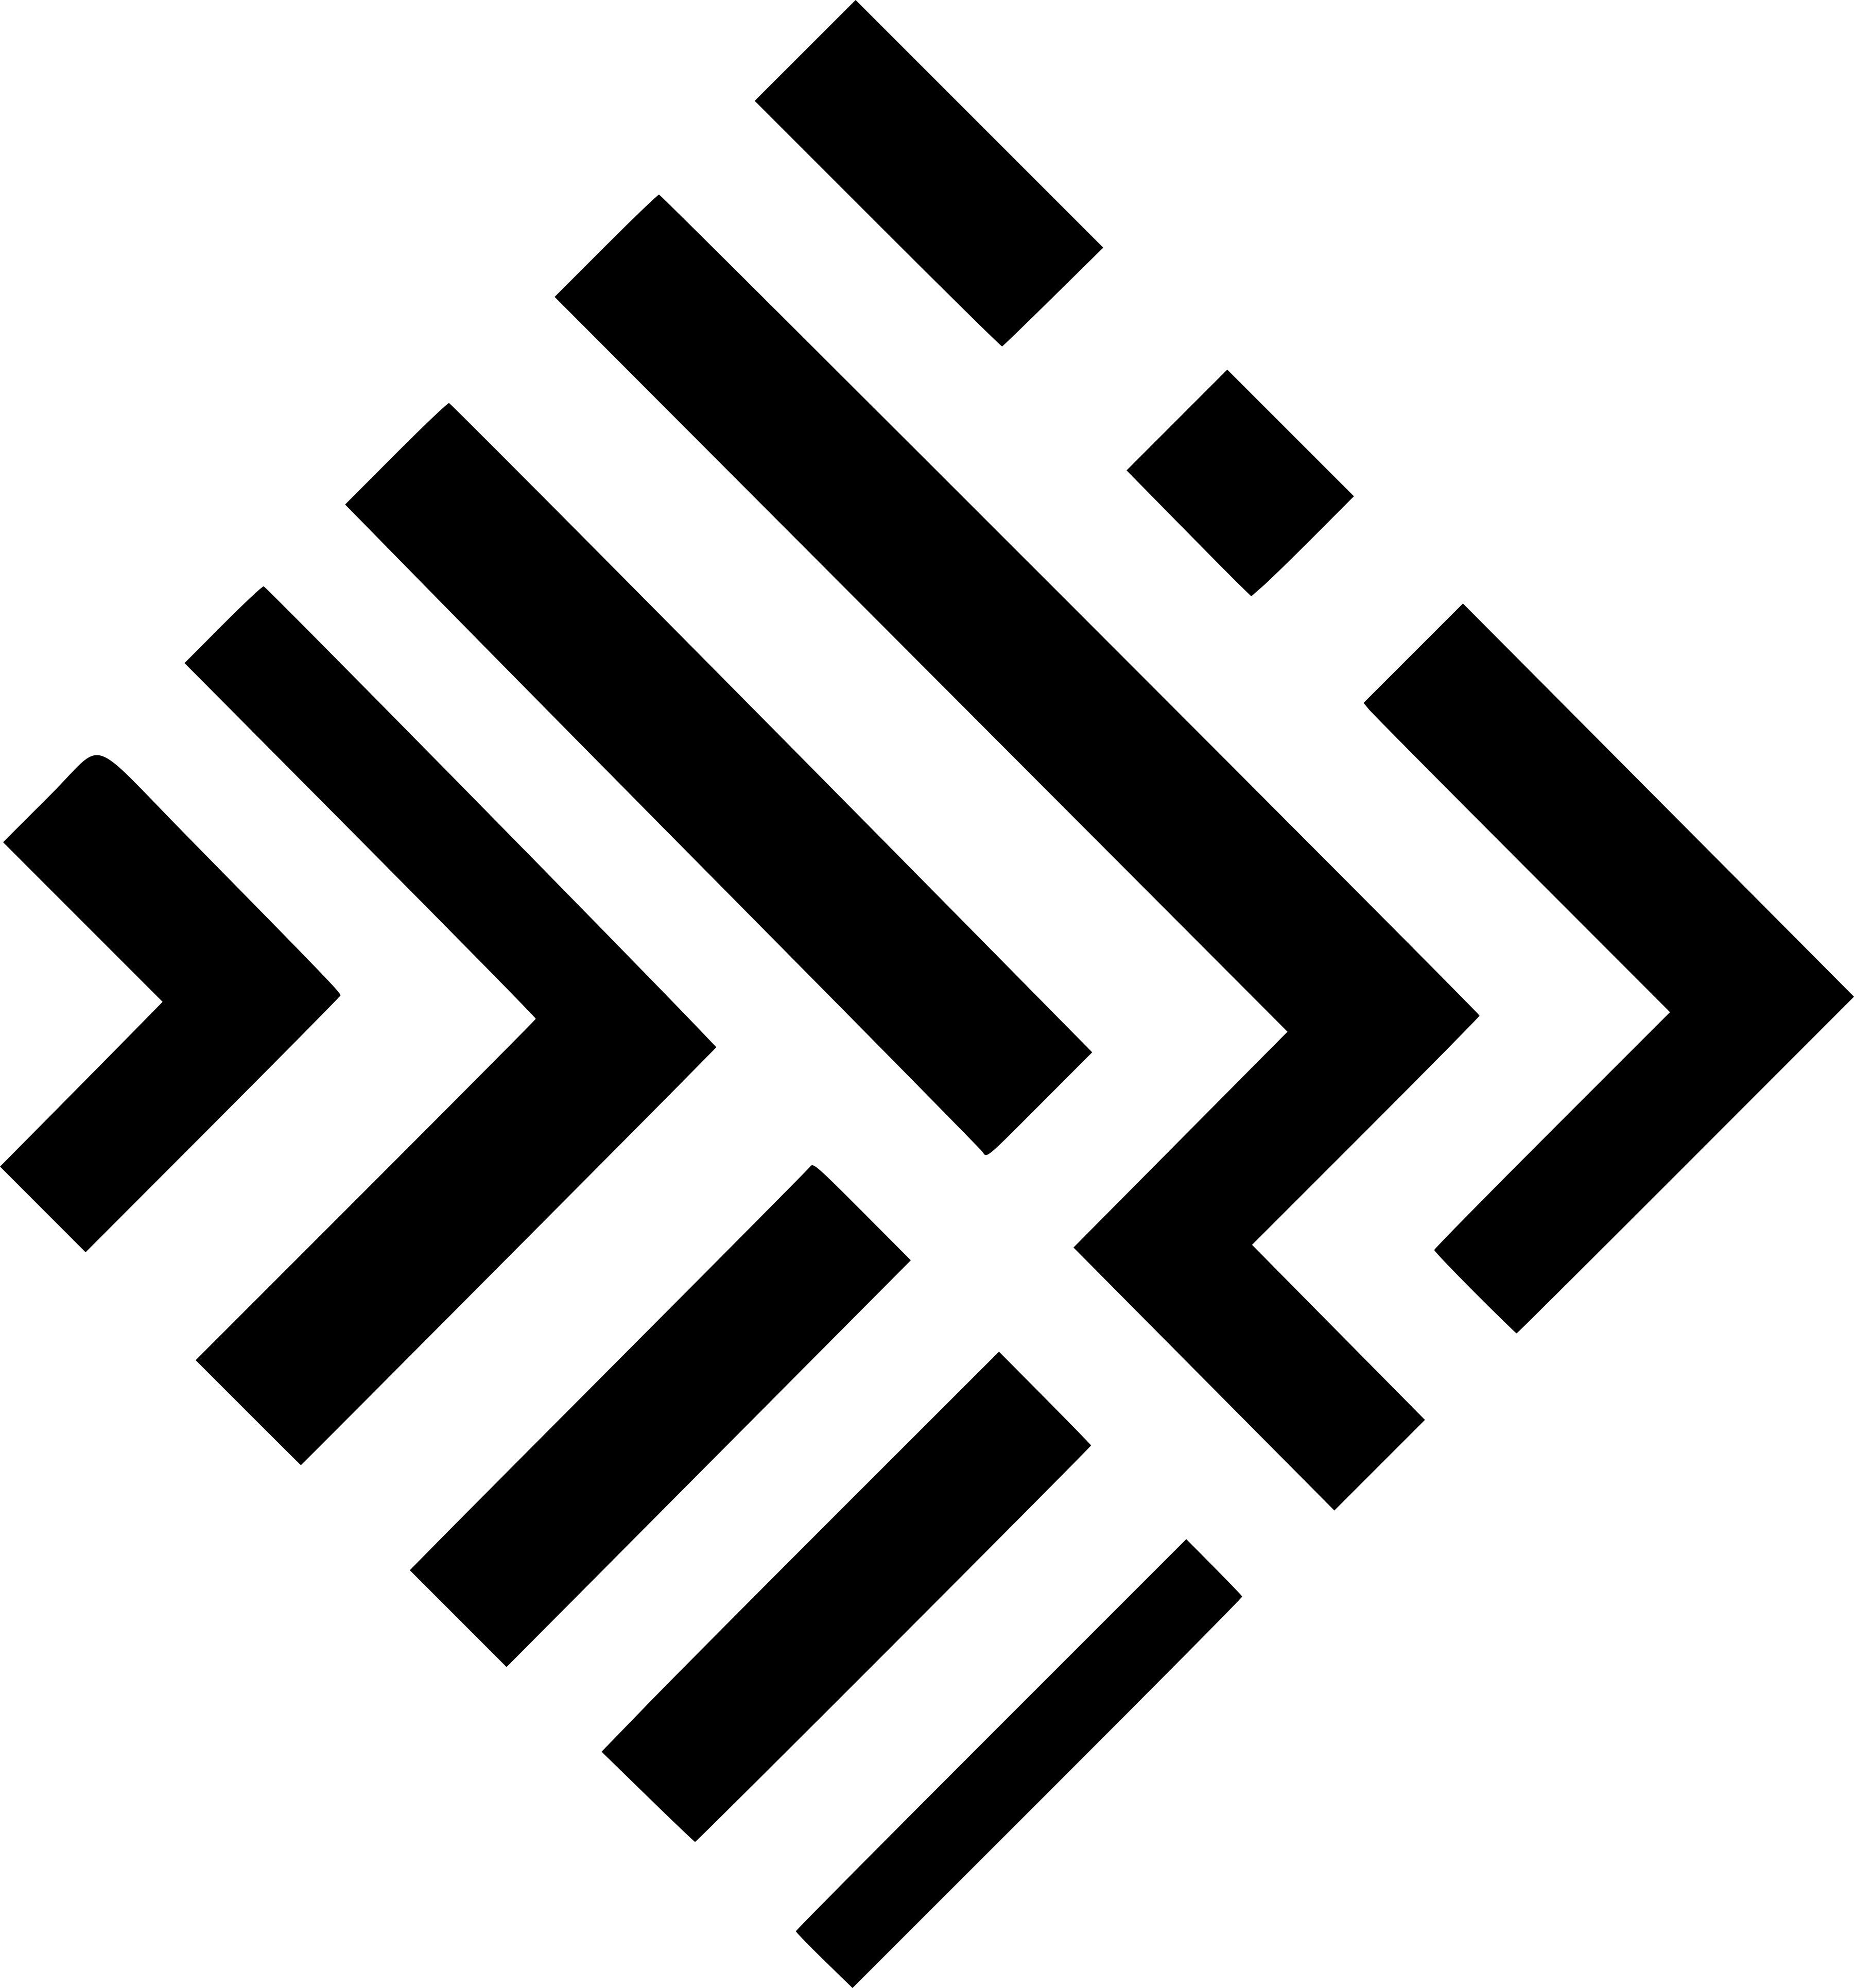
\includegraphics[height=2ex]{figures/ch3_aoc/illustrations/orthogonium_logo_b.png} SOC & & \cmark & $k + (n\frac{k}{2})$ & \cmark & \cmark & \cmark & \cmark & \cmark & \cmark \\
%         \hline
%     \end{tabular}
%     \label{tab:big_picture}
% \end{table*}


Orthogonal layers have become fundamental components in various deep learning architectures due to their unique mathematical properties, which offer benefits across multiple applications. 
For instance, robustness against adversarial attacks can be achieved by managing a model’s Lipschitz constant~\cite{szegedy_intriguing_2013} -- with 1-Lipschitz networks being a prime candidate: such networks allowing the computation of robustness certificates. 
Initially, researchers experimented with regularization techniques~\cite{cisse2017parseval}; however, constrained networks, especially those employing orthogonal layers, soon became central, as they provided the advantage of tighter certification bounds: The overall Lipschitz constant of a sequence of layers is typically estimated as the product of the individual layer constants; however, this bound is often loose, and computing the exact constant is NP-hard \cite{virmaux2018lipschitz}. \cite{anil_sorting_2019} 
shows that combining MaxMin activation with orthogonal layers makes the aforementioned bound tight.
Beyond robustness, orthogonal layers also play a key role in enhancing performance in normalizing flows. Normalizing flows are generative models that transform simple distributions into complex ones via invertible mappings \cite{dinh2016density, rezende2015variational}.  Orthogonal convolutions enable these transformations with a computable Jacobian determinant, thus improving training efficiency \cite{kingma2018glow} and forming the basis for invertible residual networks \cite{behrmann2019invertible}.
Additionally, orthogonal layers stabilize training deep and recurrent neural networks (RNNs) by preserving gradient norms through time, essential in capturing long-term dependencies in time-series, such as language and speech tasks \cite{kiani_projunn_2022,qi_deep_isometric_2020, bansal2018gainorthogonalityregularizationstraining}. Lastly, in Wasserstein GANs (WGANs) \cite{arjovsky2017wasserstein} orthogonality in both the discriminator and generator~\cite{muller2019orthogonal} supports stability and expressivity without requiring weight clipping or gradient penalties~\cite{gulrajani2017improved}, making it essential for large-scale GAN training~\cite{brock2018large, miyato2018spectral}.
See \cref{sec:ap_intro} for a detailed list of applications.


Despite these benefits, extending orthogonality to convolutional layers remains challenging. The orthogonalization of large Toeplitz matrices-structures central to convolution- is challenging to do without compromising its convolutional properties and is sometimes non-feasible~\cite {achour2023existencestabilityscalabilityorthogonal}. %\franck{Je mettrais ici un paragraphe sur le fait qu'il faut aussi supporter le stride/dilation/transpose+appendix pour plus de details}Efficient orthogonalization of these structured matrices has theoretical importance, affecting generalization~\cite{bethune_pay_2022} and indicating when orthogonal convolution is feasible~\cite{achour2023existencestabilityscalabilityorthogonal}.
%\franck{Peut etre redonner du poids au regul en mettant un \textbf{Regul}, et les mettre ds le tableau avec une croix sur orthogonal?}
Early approaches \cite{wang_orthogonal_2020, qi_deep_isometric_2020} explored regularization, yet practical constraints led to the following solutions:

\noindent \textbf{Explicit Construction Methods.} Building on \cite{xiao_dynamical_2018}, approaches like BCOP \cite{li_preventing_2019}, SC-Fac \cite{su_scaling-up_2021}, and ECO \cite{yu_constructing_2021} construct orthogonal convolutions directly in the spatial domain. These methods maintain orthogonality but often lack flexibility in kernel size control and do not support operations like striding and transposed convolutions.

\noindent \textbf{Frequency Domain Approaches.} Methods such as Cayley Convolution \cite{trockman_orthogonalizing_2021}, LOT \cite{xu_lot_2023}, and ProjUNN-T \cite{kiani_projunn_2022} enforce orthogonality by parameterizing kernels in Fourier space,
albeit at the cost of increased computational complexity and constraints on spatial or grouped convolutions.

\noindent \textbf{Composite Layer Techniques.} Skew Orthogonal Convolutions \cite{singla_skew_2021} combine multiple convolutional layers to approximate orthogonality, resulting in an orthogonal block that uses convolutions. 


\noindent \textbf{Mitigating vanishing gradients.} In some cases, strict orthogonality is relaxed. Leading to layers that are 1-Lipschitz while mitigating vanishing gradients. This avoids the computational demands of full orthogonalization~\cite{prach_almost-orthogonal_2022, meunier_dynamical_2022, araujo_unified_2023}.

\noindent Despite their success in certifiable adversarial robustness, these methods have seen limited adoption in other fields. This is largely due to implementation limitations: current layers fail to support essential features like stride, groups, or dilation, which are critical for architectures such as U-Nets~\cite{ronneberger2015u}, GANs~\cite{goodfellow2014generative}, VAEs~\cite{kingma2013auto} (upsampling convolutions), dilated CNNs~\cite{li2018csrnet} (dilation), and modern models like ResNeXt~\cite{xie2017aggregated} and EfficientNet~\cite{tan2019efficientnet} (grouped convolutions).  On the other end, performance in certifiable adversarial robustness is tied to model size and training duration \cite{prach_1-lipschitz_2023}. However, 1-Lipschitz constrained networks lack the usual scaling laws \cite{prach2024intriguing}, often requiring massive datasets even for small-scale problems \cite{hu_recipe_2023}. Developing an efficient and scalable method that supports modern features method could address both challenges simultaneously.


\paragraph{Our Contributions.}
In response to the limitations of existing methods, we introduce \textbf{A}daptive \textbf{O}rthogonal \textbf{C}onvolution (\textbf{AOC}), a method that combines two existing approaches to construct convolution layers that address the following key constraints \textit{simultaneously} while remaining efficient:
\begin{itemize}[itemsep=7pt, topsep=5pt, parsep=0pt, partopsep=0pt]
    \item \textbf{Orthogonal}: AOC enforces strict orthogonality, allowing convolutional layers to retain essential properties across applications.     
    \item \textbf{Explicit}: In contrast to frequency domain methods, AOC generates explicit convolution kernels in the spatial domain, allowing straightforward implementation in standard deep learning frameworks without specialized operations or significant computational overhead. 
    \item \textbf{Flexible}: Supporting a range of essential operations -- including striding, transposed convolutions for upsampling, grouped convolutions, and dilation -- AOC adapts effectively to modern neural network architectures.
    \item \textbf{Scalable}: Designed for large-scale applications, our implementation maintains efficiency, incurring only a 10\% slowdown compared to unconstrained models in realistic ImageNet 1K~\cite{deng2009imagenet} training setup.
\end{itemize}
To underscore the advantages of our method, we include a comparative summary in  \cref{tab:big_picture}, highlighting support for key features across different methods.
By combining orthogonality, explicit construction, and flexibility, our approach seamlessly bridges theoretical rigor with practical efficiency in deep learning models. Beyond AOC, this work introduces a mathematical framework that unlocks improvements of other existing methods such as SOC, SLL, or Sandwich (See \cref{sec:ap_improving_existing}). Our implementation was rigorously tested and is available in a package called \fulllibname, which also contains improved implementations of other existing methods.


The paper is organized as follows:  \Cref{sec:AOC} outlines the three main aspects of AOC -- its core tools, kernel construction, and scalable implementation. \Cref{sec:eval} presents an evaluation of the method's performance in terms of speed and expressive power. Finally, \cref{sec:conclusions} discusses how our approach can enhance existing methods in the literature.
